\label{sec:testbed}

We proceed to define the testbed environment by each of its conforming
parts. We later indicate a procedure to set up the testbed. In this procedure,
we summarize all the details regarding on setting the connectivity and
system files for a set of \ac{Raspi}s in a centralized fashion.
Afterwards, we indicate how to cross-compile the Kodo library in an
easy way. Finally, we provide further information about Kodo itself in terms
of testing, other platforms supported and source code documentation
for further references.

\subsection{System Overview}


\begin{figure}[ht!]
\centering
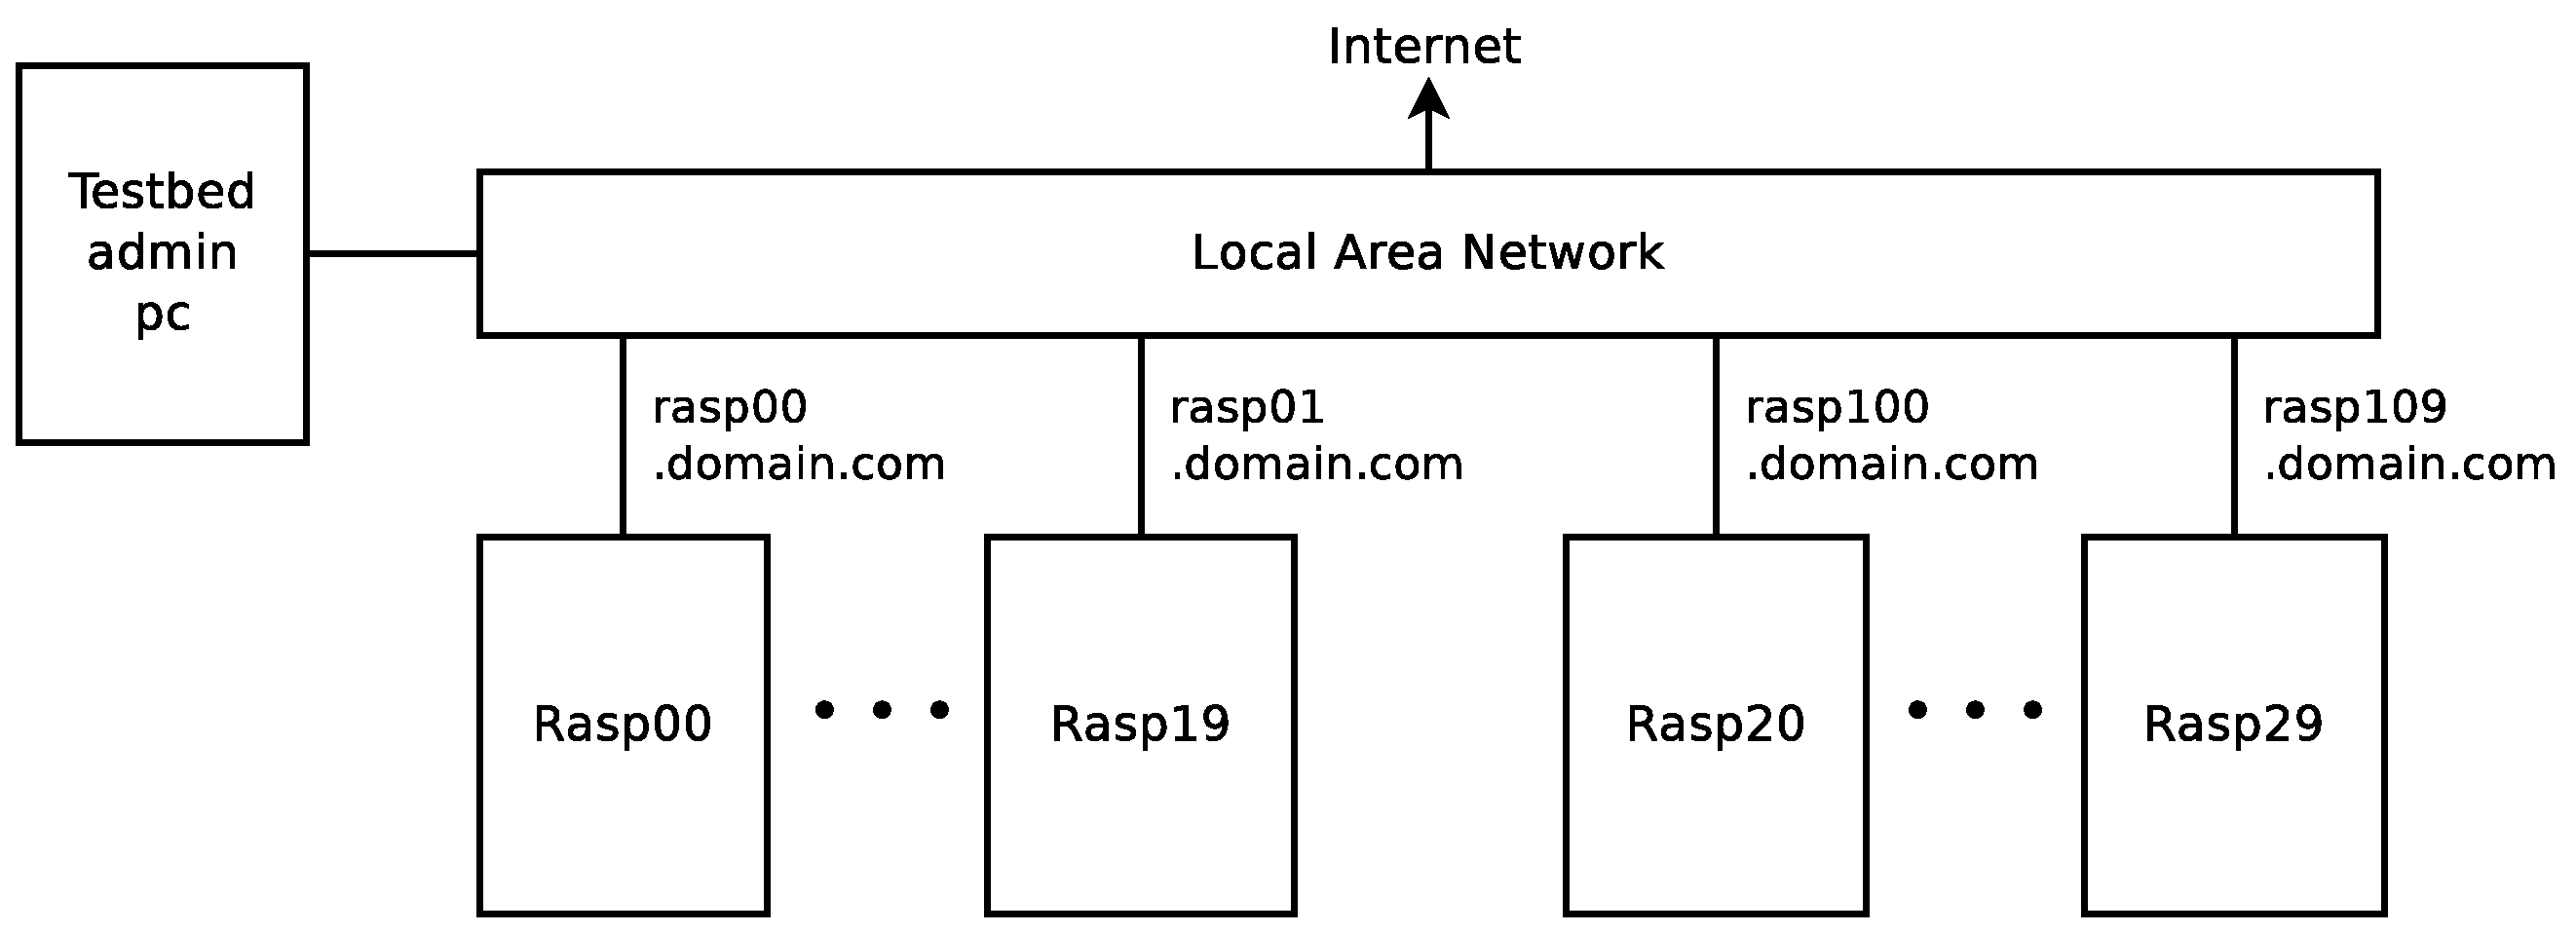
\includegraphics[width=0.6\textwidth]{images/testbed_setup2.eps}
\caption{Testbed setup}
\label{fig:testbed_setup}
\end{figure}

This section will present a testbed of thirty \ac{Raspi}s.
%Twenty \ac{Raspi} 1 model B revision 2 and ten \ac{Raspi} 2 model B V1.1.
They are all equipped with a memory card and are connected to the
university network by wire using their ethernet interface (eth0).

To easily discover the \ac{Raspi}s within the university network, they have all
been assigned a unique name under a common domain.
This eliminates the need to remember their individual \ac{IP}s.

A sketch of the testbed is depicted in figure~\ref{fig:testbed_setup}.
We have two types of \ac{Raspi}s in our setup.
Table \ref{tab:rasp_naming} shows the naming convention.

\begin{table}[ht!]
  \centering
  \begin{tabular}{|c|c|}
    \hline
      \textbf{Hostname} & \textbf{Model} \\ \hline
    Rasp00 - Rasp19 & Raspberry Pi 1 model B rev. 2 \\ \hline
    Rasp100 - Rasp109 & Rasperry Pi 2 model B V1.1 \\ \hline
  \end{tabular}
  \caption{Raspberry Pi naming convention}
  \label{tab:rasp_naming}
\end{table}




Accessing them is easily done using \ac{SSH}.
To address them within the university network,
The \ac{Raspi}s

The \ac{Raspi}s are all equipped with an ethernet interface (eth0) and
connected by wire to the university's \ac{LAN}. The university network
administration was provided
the \ac{MAC} addresses of the ethernet interfaces to automatically assign
the devices the desired \ac{IP} addresses as shown in the figure. In a personal
\ac{LAN}, another option could be to manually provide the devices with static
\ac{IP}s.


This section will be used to present a \ac{Raspi} testbed and the steps to
install and configure its devices.

The testbed is depicted in figure~\ref{fig:testbed_setup}. It consists of twenty
Raspberry Pi 1 model B rev 2 (Rasp01 to Rasp20) and
ten Raspberry Pi 2 model b V1.1 (Rasp2\_01 to Rasp2\_10).

The goal is to configure all the \ac{Raspi}s identically with the same software
and configurations. There are however a few differences between them that we
need to take into account. E.g. hostname and network addresses.

The testbed will be used by students that might need to change how the
devices are work either temporary or permanently. We will illustrate how this
can be accomplished using an overlaying filesystem.

Finally, it should be possible to store data that are generated from
simulations on the memory cards that are in the individual \ac{Raspi}.
%We using a overlaying filesystem that
%We will illustrate
%how that can be done. In the case of temporary changes, it is important that
%all changes can be easily reverted. We put a \ac{RAM} filesystem on top of
%the the root filesystem to .
%the configure the
%devices to behave according to their test specifications. We
%will also present how that might be done.

%their linkings. That could be to change network config

%The goal is to configure all the devices to be as identical as possible. This
%means that it is desired to have the same software on every device, but

The \ac{Raspi}s are all equipped with an ethernet interface (eth0) and
connected by wire to the university's \ac{LAN}. The university network
administration was provided
the \ac{MAC} addresses of the ethernet interfaces to automatically assign
the devices the desired \ac{IP} addresses as shown in the figure. In a personal
\ac{LAN}, another option could be to manually provide the devices with static
\ac{IP}s.
%that are
%assigned the \ac{IP} addresses in the figure and connected wired to the
%university's \ac{LAN}.

We use standard usb power adapters to power the \ac{Raspi}s.

\subsubsection{Installing Raspbian}

To get started, we first need to install an \ac{OS} on the
Raspberry Pis. We will use Raspbian linux~\cite{raspbian}

We will use a desktop that has linux installed to download,
configure, and write the image to the memory cards.
%We have decided to use a linux desktop machine to create a
%common image of Raspbian Linux that can be used in any of the Raspberry Pis.

%for all devices. After the image has been configured it can be written to
%a memory card and used in any of the Raspberry Pis. This means that each
%device needs a memory card, but it does not matter which card is put into
%which device.

We have decided to go with Raspbian linux~\cite{raspbian} and
to install it on memory cards.


%There exists a number of ways to setup a testbed in a centralized manner.
%E.g. using e.g. \ac{NFS}.

There exists a number of ways to setup a testbed

with multiple devices. We
have decided on a very simple approach of simply instal


-
- Download image (wget)
- Update/Modify image (chroot)
- Burn image
- Bang! linux is running
-

Open a terminal, and then...

hashmark (\#) means to perform operation as root, dollar (\$) means to perform operation as user


The first thing we need to do is to download the linux installation file.
For Raspbian, this is available at \url{http://downloads.raspberrypi.org}.

Raspbian is made available in two bundles. Raspbian and Raspbian lite.
The difference between the two is that Raspbian contains a pre-installed desktop
environment, and Raspbian lite is by default only accessable through a shell. 
They will both also be remotely accessible using \ac{SSH}.

Our testbed does not have monitors so we will install Raspbian lite.
A desktop environment can always be installed manually in case that will be
desired sometime in the future.

Below is a procedure of how we setup the \ac{Raspi}s in our testbed. We
have decided a simple setup where each \ac{Raspi} is equipped with a
memory card that contains a slightly customized Raspbian lite image with
identical settings. 

The reason this can be done easily is because the official Raspbian lite image
that we will download simply conntains a complete linux installation that are
packaged in an image rather than written to a harddrive, memory card, or usb
pen.

The overall steps to customize the official Raspbian lite image are listed below:
\begin{enumerate}
    \item Download Raspbian lite
    \item Alter Raspbian lite. E.g. browse, modify, add, and delete files
        in the official Raspbian lite image
    \item Change root. I.e. change root filesystem into the Raspbian lite
        image to update and install software packages
    \item Write image to memory cards
\end{enumerate}

\subsection{Download Raspbian lite}

To download the latest Raspbian lite, we go to the url
\url{http://downloads.raspberrypi.org/raspbian_lite/images/}.
At the time of this writing, the latest bundle was
2016-05-27-raspbian-jessie-lite.zip.

We want to proceed downloading the image with a shell instead of the browser.
To do this, first open a command window on a linux machine. This guide is
assuming a debian based distribution, but there should only be minor differences
if you have another package manager. I.e. the application that is used to
download and install software packages in linux.

After the terminal has been opened, we first declare a few variables to reduce
redundant typing. The first variables we declare is the Raspbian image name.
Notice that the extension has been omitted. This is because the image has been
packed into a zip file.
The other variable we declare is a working directory. This is where we will
download the image to and work on it. In other words, it will be stored in
/home/<username>/Raspbian

%To download Raspbian lite, we go to the \url{http://downloads.raspberrypi.org}.
%There should be a folder called raspbian\lite and
%to find the download page at which Raspbian lite should be located. Instead of
%downloading with the browser, we just extract the download url to the latest
%image. At the time of this writing, that was

% Define variable]
\begin{lstlisting}[]
$ export IMAGE="2016-05-27-raspbian-jessie-lite"
$ export WORKDIR="${HOME}/Raspbian"
\end{lstlisting}
\FloatBarrier

A final thing to notice is the way \$ and \# are used in the code blocks. \$
means that the command can be run as a normal user where \# indicates that the
command should be run with root permissions.
Running a command with root permissions can on most systems be done by putting
the command "sudo" in front of each line. This is illustrated in the code below
with the command "whoami" that prints the username of the caller. Lines without
leading \$ or \# is the terminal output.

% Root example
\begin{lstlisting}[]
$ whoami
chres
$ sudo whoami
root
\end{lstlisting}
\FloatBarrier

Next, we make the working directory and change directory (cd) into the working
directory. We can then use wget to download Raspbian lite. Unpack the image
when the download is complete.

% Download and unpack image
\begin{lstlisting}[]
$ mkdir -p ${WORKDIR}
$ cd ${WORKDIR}
$ wget http://downloads.raspberrypi.org/raspbian_lite/images/raspbian_lite-2016-05-31/${IMAGE}.zip
$ unzip ${IMAGE}.zip
\end{lstlisting}
\FloatBarrier

\subsection{Mount image}

After Raspbian lite has been unpacked, there should be an .img file in the directory.
"fdisk" can be used to display what is inside. Pass the arguments "-u sectors" to
display the sizes in sectors and "-l" to display partitions and exit.

% Check out the image   % The dollar hack was to fix vim syntax
\begin{lstlisting}[literate={DOLLAR}{\$}1]
DOLLAR fdisk -u sectors -l ${IMAGE}.img
Disk 2016-05-27-raspbian-jessie-lite.img: 1.3 GiB, 1387266048 bytes, 2709504 sectors
Units: sectors of 1 * 512 = 512 bytes
Sector size (logical/physical): 512 bytes / 512 bytes
I/O size (minimum/optimal): 512 bytes / 512 bytes
Disklabel type: dos
Disk identifier: 0x6fcf21f3

Device                               Boot  Start     End Sectors  Size Id Type
2016-05-27-raspbian-jessie-lite.img1        8192  137215  129024   63M  c W95 FAT32 (LBA)
2016-05-27-raspbian-jessie-lite.img2      137216 2709503 2572288  1.2G 83 Linux
\end{lstlisting}
\FloatBarrier

The image contains two partitions. The first one of starting at sector 8192 and
the other partition starting at sector 137216. The partitions is of type FAT32
and Linux and have sizes 63M and 1.2G. This indicates that the first partition
is most likely a boot partition and the second partition is a traditional file
system. Actually, it is a linux root filesystem (i.e. /).



%We see that the boot and root partitions starts at sector 8192 and 137216 respectivly.
%We also notice that each sector is 512 bytes.


%On newer systems, we can mount the device easier using "losetup --show -f -P IMAGE"

%Mount root partition:

To browser and alter the files in the image, it is possible to mount the partitions.

Lets first mount the root partition. This is done by first creating a new folder
that we will call root which will be located in our working directory. After this,
we mount the partition starting at sector 137216. To provide this offset information
to mount, we need to find the offset in bytes. From the fdisk command we could also
see that each sector is 512 bytes. Thus, we multiply the sector size and the sector
start to get the offset in bytes.

\begin{lstlisting}[]
$ export ROOTDIR="${WORKDIR}/root"
$ mkdir -p ${ROOTDIR}
# mount -o loop,offset=$((137216*512)) ${IMAGE}.img ${ROOTDIR}
\end{lstlisting}
\FloatBarrier

After this, we can also mount the boot partition inside the newly mounted
root filesystem. This is useful because that partition will be mounted
this exact place when a \ac{Raspi} starts up with a memory card containing
this image. It is therefore the natural place to mount it for later purposes.

Mount boot partition:
\begin{lstlisting}[]
# mount -o loop,offset=$((8192*512)) ${IMAGE}.img ${ROOTDIR}/boot
\end{lstlisting}
\FloatBarrier

We can now change all the files in the disk image.



\subsection{Configuring OS files and scripts}


% MAC and Hostname file
\Suppressnumber\begin{lstlisting}[]
<@\textcolor{gray}{\$\{ROOTDIR\}/home/pi/rasp\_config/nodes.csv}@>
<@\textcolor{gray}{
---------------------------------------------------------------}
\Reactivatenumber @>
# Ethernet MAC    Hostname
b8:27:eb:5b:da:20 rasp00
b8:27:eb:7b:c3:91 rasp01
b8:27:eb:54:9c:64 rasp02
b8:27:eb:95:bd:11 rasp03
\end{lstlisting}
\FloatBarrier


% Set hostname
\Suppressnumber\begin{lstlisting}[]
<@\textcolor{gray}{\$\{ROOTDIR\}/home/pi/rasp\_config/set\_hostname}@>
<@\textcolor{gray}{
---------------------------------------------------------------}
\Reactivatenumber @>
#!/usr/bin/env bash
mac=$(cat /sys/class/net/eth0/address)
hostname=$(grep $mac nodes.csv | cut -f2 -d' ')

# Assign hostname found in nodes.csv
if [ ! -z $hostname ]; then
    echo $hostname > /etc/hostname
    hostname $hostname
fi
\end{lstlisting}
\FloatBarrier



% Get the files
\begin{lstlisting}[]
$ wget http://kom.aau.dk/project/TuneSCode/rasp_config.zip
# unzip rasp_config.zip -d ${ROOTDIR}/home/pi/
\end{lstlisting}
\FloatBarrier


Call set\_hostname script at startup. We insert a line of code to call script in rc.local just after the initial comments (i.e. lines starting with \#).
\begin{lstlisting}[]
# line_number=$(egrep -n -m1 "(^[^#])|(^$)" ${ROOTDIR}/etc/rc.local | cut -d: -f1)
# sed -i "${line_number}c bash /home/pi/rasp_config/set_hostname" ${ROOTDIR}/etc/rc.local
\end{lstlisting}
\FloatBarrier
%$ line="bash /home/pi/.rasp_config/set_hostname"
%# awk -v text="$line" '!/^#/ && !p {print text; p=1} 1' ${ROOTDIR}/etc/rc.local > <@ \Suppressnumber @>
%    ${ROOTDIR}/etc/rc.local <@ \Reactivatenumber @>


All other files could be updated.

\subsection{Installation and Updating the image}

It may be desired to pre-install some programs in the image before it is
written to all the memory cards that goes into the Raspberry pis.
This can be done using QEMU Chroot (change root).
\url{https://wiki.archlinux.org/index.php/Raspberry_Pi}

\fxnote{Lets use RPi for Raspberry Pis throughout the paper!}
\fxnote{Which packages is required for this on debian/ubuntu?}


% CHROOT to OS image
\begin{lstlisting}[]
# apt-get install binfmt-support qemu qemu-user-static
# update-binfmts --importdir /var/lib/binfmts/ --import
# update-binfmts --display qemu-arm
# update-binfmts --enable qemu-arm
\end{lstlisting}
\FloatBarrier

% CHROOT to OS image
\begin{lstlisting}[]
# cd $ROOTDIR
# cp /etc/resolv.conf etc/resolv.conf
# cp /usr/bin/qemu-arm-static usr/bin
# mount -t proc proc proc/
# mount --rbind /sys sys/
# mount --rbind /dev dev/
# proot -q qemu-arm-static -S ${ROOTDIR}

ALTERNATIVE:
# chroot ${ROOTDIR} /usr/bin/qemu-arm-static /bin/bash
\end{lstlisting}
\FloatBarrier


% Optionally, we may create a unique prompt to indicate we have changed root
\begin{lstlisting}[]
# export PS1="(chroot) $PS1"
\end{lstlisting}
\FloatBarrier



% Update system
\begin{lstlisting}[]
# apt-get update
# apt-get upgrade
\end{lstlisting}
\FloatBarrier

Lets install some programs
% Install packages
\begin{lstlisting}[]
# apt-get install vim git
\end{lstlisting}
\FloatBarrier



\subsection{Installation an overlaying filesystem}

We use the code provided by

Assumuing that we are still chrooted to the RPi image and the boot partition is mounted to /boot

% Get files
\begin{lstlisting}[]
# OVERLAYROOTDIR="/tmp/overlayroot"
# git clone https://github.com/chesty/overlayroot.git $OVERLAYROOTDIR
\end{lstlisting}
\FloatBarrier

% Install required packages
\begin{lstlisting}[]
# apt-get install busybox
\end{lstlisting}
\FloatBarrier

% Setup initramfs
\begin{lstlisting}[]
# cp ${OVERLAYROOTDIR}/hooks-overlay /etc/initramfs-tools/hooks/
# cp ${OVERLAYROOTDIR}/init-bottom-overlay /etc/initramfs-tools/scripts/init-bottom/
# echo "overlay" > /etc/initramfs-tools/modules
\end{lstlisting}
\FloatBarrier

% Tell uboot to load initramfs
\begin{lstlisting}[]
# echo "initramfs init.gz" > /boot/config.txt
\end{lstlisting}
\FloatBarrier

% Create an initramfs
\begin{lstlisting}[]
# How to i know the kernel version /lib/modules/
# mkinitramfs -o /boot/init.gz -k 4.4.11+
\end{lstlisting}
\FloatBarrier

\subsection{Write image}

% Exit chroot, umount, and write to memory card
\begin{lstlisting}[]
# exit
# cd ..
# umount --recursive ${ROOTDIR}
# losetup -d WHICH_NUMBE.img
# dd if=${IMAGE}.img of=/dev/mmcblk0 bs=4M
\end{lstlisting}
\FloatBarrier

How about kodo python?

\subsection{fabric}

% Exit chroot, umount, and write to memory card
\begin{lstlisting}[]
from fabric.api import run, env, task
# Python Fabric script to run commands on multiple hosts through ssh
#
# Run script as 'fab <task>', where <task> is one of the scripts functions
# marked as a tesk. The task marked as 'default' will be run if <task> is not
# specified

env.hosts = ['rasp00.domain.com','rasp01.domain.com','rasp02.domain.com']
env.user = 'root'
env.password = 'sdn'

@task
def install(program):
    """
    Install a program
    program: program name
    """
    result = run('apt-get install -y {}'.format(program), quiet=True)

@task
def copy_to_rasp(filename):
    put(...)

\end{lstlisting}
\FloatBarrier

execute a script function by calling "fab install:feh"

\subsection{Kodo cross-compilation: From your PC to the Raspberry Pi}

Besides the previous description (\textbf{Include compiling Kodo from the
RasPi from the scratch}), the testbed administrator can compile Kodo in its
personal workstation and transfer the generated binaries directly to
a path in the \ac{Raspi}. To achieve this, we get a toolchain that
contains the binaries for the \texttt{raspberry-gxx49-arm-g++} compiler
for the \ac{Raspi}. Therefore, we strongly recommend any testbed
administrator to do the following procedure. In what follows, we provide
the instructions considering that the NFS server uses the \texttt{\$HOME}
directory as the working directory. However, the administrator may choose
some other working directory of its preference if desired.

\begin{enumerate}

\item Download the \ac{Raspi} toolchain for 64-bit Linux from: \\
\texttt{http://buildbot.steinwurf.dk/toolchains/linux/} to your
\texttt{\$HOME} directory. \\

\item Extract the downloaded file locally in the NFS server. After
this operation, there should be a new directory for the toolchain
in the server. \\

\item Add the \texttt{bin} folder of the toolchain to the \texttt{PATH}
Linux environment variable of the server. This will help the server OS
to recognize the location of the compiler command, which will be needed
later. To do so, edit the \texttt{\$HOME/.profile} to add in a newline:
\texttt{PATH="\$PATH:\$HOME/raspberry-gxx49-arm/bin"}. Save the
\texttt{\$HOME/.profile}. \\

\item Restart the server session in order for the changes made in the
previous step take effect. To verify this, open a new terminal and type:
\texttt{raspberry-gxx49-arm-g++ --version}. A correct binary installation
should return an output similar to:

\texttt{raspberry-gxx49-arm-g++ (crosstool-NG 1.21.0) 4.9.3 20150311 (prerelease)
Copyright (C) 2014 Free Software Foundation, Inc.
This is free software; see the source for copying conditions.  There is NO
warranty; not even for MERCHANTABILITY or FITNESS FOR A PARTICULAR PURPOSE.} \\

\item Clone the Kodo repository in the server by executing: \\
\texttt{git clone git://github.com/steinwurf/kodo.git} in \texttt{\$HOME}.
\textbf{Change the repo to kodo-rlnc or kodo-cpp since just raw kodo is going
to be depreceated soon} \\

\item Navigate to the repository and configure \texttt{waf} by typing:
\texttt{python config.py} and select the 16th ``make specification'' file
for the \ac{Raspi}, e.g. option \texttt{[16]cxx\_raspberry\_gxx49\_arm}
presented by the file.

This command configures \texttt{waf} to use the proper compiler and its
required flags to generate the binaries for the \ac{Raspi}. If the
configuration was correct, the output will indicate:
\texttt{'configure' finished successfully (X.XXXs)}, where \texttt{X.XXX}
is total time in seconds for configuring the project in the server. \\

\item Execute \texttt{python waf build}. If the build process was
successful, the generated binaries for the \ac{Raspi} should be located
in \texttt{build/cxx\_raspberry\_gxx49\_arm} in the Kodo repository.
\textbf{Indicate how the binary files should look like}.

Once this procedure is made, the testbed administrator can relocate the
generated binary files to the \ac{Raspi}s through the network as desired
by using the \texttt{scp} command during the configuration step.


\end{enumerate}

\subsection{Kodo Builds for the \ac{Raspi}, Platform Support and Documentation}

You can check the build status of Kodo, Fifi and other relevant projects
through their respective repository master branch on our buildbot page
\cite{steinwurf2016buildbot}. Our buildbot displays the status of the builds
for Raspbian 8 and GCC 4.9 for the ARM architecture which is the relevant one
for the \ac{Raspi}. At the link, you can check build status and build
statistics. Also, documentation about Kodo basics with a tutorial is available
at \cite{kododocs}.
